\documentclass[tikz,border=5pt]{standalone}
\usepackage{fontspec}
\setmainfont{TeX Gyre Termes}
\setsansfont{TeX Gyre Heros}
\usepackage{pgfplots}
\pgfplotsset{compat=1.18}
\usetikzlibrary{patterns,positioning,arrows.meta}
\definecolor{blue}{HTML}{0072B2}
\definecolor{green}{HTML}{009E73}
\definecolor{orange}{HTML}{E69F00}
\definecolor{red}{HTML}{D55E00}
\definecolor{grey}{HTML}{8D9399}
\pgfplotsset{every axis/.append style={width=8.1cm,height=5.3cm,
font=\small,axis lines=left,axis line style={grey},tick align=outside,
enlarge x limits=.18,ymajorgrids=true,grid style={grey!18},
tick label style={font=\small},label style={font=\small},
nodes near coords style={font=\small,/pgf/number format/fixed,/pgf/number format/precision=2,/pgf/number format/1000 sep={,}},clip=false}}
\begin{document}
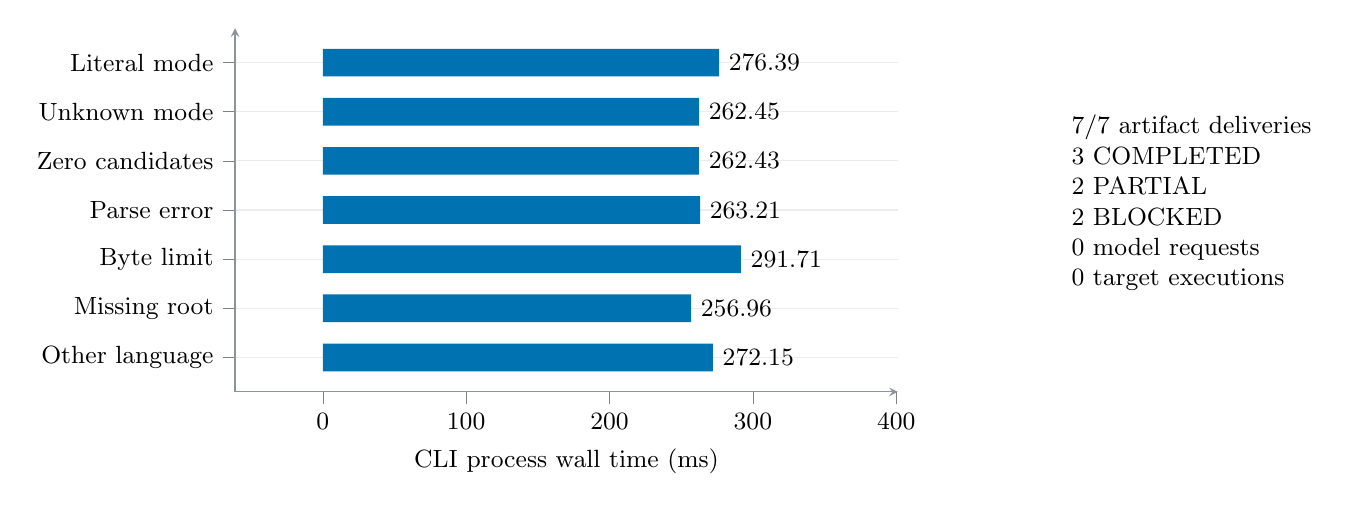
\begin{tikzpicture}
\begin{axis}[xbar,width=10cm,height=6.2cm,xmin=0,xmax=340,ymin=-.7,ymax=6.7,ytick={6,5,4,3,2,1,0},yticklabels={Literal mode,Unknown mode,Zero candidates,Parse error,Byte limit,Missing root,Other language},xlabel={CLI process wall time (ms)},nodes near coords,point meta=x]
\addplot[fill=blue,draw=none] coordinates {(276.39,6) (262.45,5) (262.43,4) (263.21,3) (291.71,2) (256.96,1) (272.15,0)};
\end{axis}
\node[align=left,anchor=west,font=\small] at (10.5cm,2.4cm) {7/7 artifact deliveries\\3 COMPLETED\\2 PARTIAL\\2 BLOCKED\\0 model requests\\0 target executions};\end{tikzpicture}
\end{document}
